% Created by tikzDevice version 0.12 on 2019-01-19 16:45:01
% !TEX encoding = UTF-8 Unicode
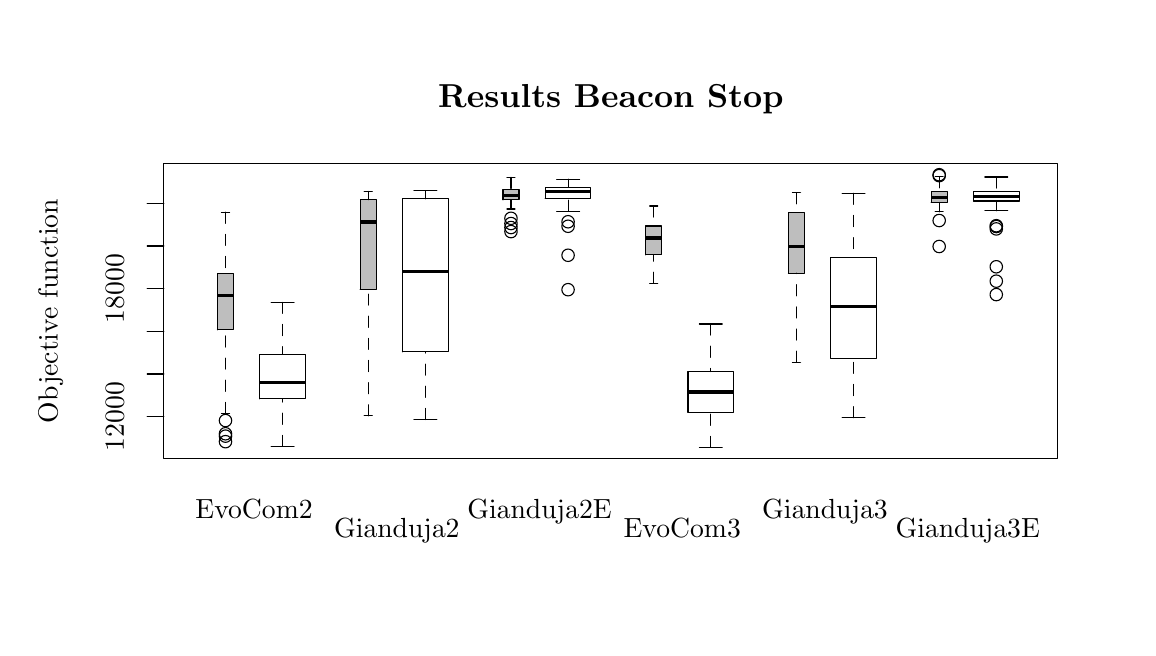
\begin{tikzpicture}[x=1pt,y=1pt]
\definecolor{fillColor}{RGB}{255,255,255}
\path[use as bounding box,fill=fillColor,fill opacity=0.00] (0,0) rectangle (397.48,216.81);
\begin{scope}
\path[clip] ( 49.20, 61.20) rectangle (372.28,167.61);
\definecolor{fillColor}{RGB}{190,190,190}

\path[fill=fillColor] ( 68.59,107.63) --
	( 74.37,107.63) --
	( 74.37,127.99) --
	( 68.59,127.99) --
	cycle;
\definecolor{drawColor}{RGB}{0,0,0}

\path[draw=drawColor,line width= 1.2pt,line join=round] ( 68.59,120.03) -- ( 74.37,120.03);

\path[draw=drawColor,line width= 0.4pt,dash pattern=on 4pt off 4pt ,line join=round,line cap=round] ( 71.48, 77.42) -- ( 71.48,107.63);

\path[draw=drawColor,line width= 0.4pt,dash pattern=on 4pt off 4pt ,line join=round,line cap=round] ( 71.48,150.13) -- ( 71.48,127.99);

\path[draw=drawColor,line width= 0.4pt,line join=round,line cap=round] ( 70.04, 77.42) -- ( 72.93, 77.42);

\path[draw=drawColor,line width= 0.4pt,line join=round,line cap=round] ( 70.04,150.13) -- ( 72.93,150.13);

\path[draw=drawColor,line width= 0.4pt,line join=round,line cap=round] ( 68.59,107.63) --
	( 74.37,107.63) --
	( 74.37,127.99) --
	( 68.59,127.99) --
	( 68.59,107.63);

\path[draw=drawColor,line width= 0.4pt,line join=round,line cap=round] ( 71.48, 74.84) circle (  2.25);

\path[draw=drawColor,line width= 0.4pt,line join=round,line cap=round] ( 71.48, 70.07) circle (  2.25);

\path[draw=drawColor,line width= 0.4pt,line join=round,line cap=round] ( 71.48, 67.21) circle (  2.25);

\path[draw=drawColor,line width= 0.4pt,line join=round,line cap=round] ( 71.48, 69.21) circle (  2.25);
\definecolor{fillColor}{RGB}{255,255,255}

\path[fill=fillColor] ( 83.86, 82.65) --
	(100.37, 82.65) --
	(100.37, 98.77) --
	( 83.86, 98.77) --
	cycle;

\path[draw=drawColor,line width= 1.2pt,line join=round] ( 83.86, 88.50) -- (100.37, 88.50);

\path[draw=drawColor,line width= 0.4pt,dash pattern=on 4pt off 4pt ,line join=round,line cap=round] ( 92.11, 65.51) -- ( 92.11, 82.65);

\path[draw=drawColor,line width= 0.4pt,dash pattern=on 4pt off 4pt ,line join=round,line cap=round] ( 92.11,117.55) -- ( 92.11, 98.77);

\path[draw=drawColor,line width= 0.4pt,line join=round,line cap=round] ( 87.99, 65.51) -- ( 96.24, 65.51);

\path[draw=drawColor,line width= 0.4pt,line join=round,line cap=round] ( 87.99,117.55) -- ( 96.24,117.55);

\path[draw=drawColor,line width= 0.4pt,line join=round,line cap=round] ( 83.86, 82.65) --
	(100.37, 82.65) --
	(100.37, 98.77) --
	( 83.86, 98.77) --
	( 83.86, 82.65);
\definecolor{fillColor}{RGB}{190,190,190}

\path[fill=fillColor] (120.17,122.27) --
	(125.95,122.27) --
	(125.95,154.64) --
	(120.17,154.64) --
	cycle;

\path[draw=drawColor,line width= 1.2pt,line join=round] (120.17,146.63) -- (125.95,146.63);

\path[draw=drawColor,line width= 0.4pt,dash pattern=on 4pt off 4pt ,line join=round,line cap=round] (123.06, 76.54) -- (123.06,122.27);

\path[draw=drawColor,line width= 0.4pt,dash pattern=on 4pt off 4pt ,line join=round,line cap=round] (123.06,157.62) -- (123.06,154.64);

\path[draw=drawColor,line width= 0.4pt,line join=round,line cap=round] (121.62, 76.54) -- (124.50, 76.54);

\path[draw=drawColor,line width= 0.4pt,line join=round,line cap=round] (121.62,157.62) -- (124.50,157.62);

\path[draw=drawColor,line width= 0.4pt,line join=round,line cap=round] (120.17,122.27) --
	(125.95,122.27) --
	(125.95,154.64) --
	(120.17,154.64) --
	(120.17,122.27);
\definecolor{fillColor}{RGB}{255,255,255}

\path[fill=fillColor] (135.44, 99.69) --
	(151.94, 99.69) --
	(151.94,154.92) --
	(135.44,154.92) --
	cycle;

\path[draw=drawColor,line width= 1.2pt,line join=round] (135.44,128.75) -- (151.94,128.75);

\path[draw=drawColor,line width= 0.4pt,dash pattern=on 4pt off 4pt ,line join=round,line cap=round] (143.69, 75.23) -- (143.69, 99.69);

\path[draw=drawColor,line width= 0.4pt,dash pattern=on 4pt off 4pt ,line join=round,line cap=round] (143.69,157.92) -- (143.69,154.92);

\path[draw=drawColor,line width= 0.4pt,line join=round,line cap=round] (139.56, 75.23) -- (147.82, 75.23);

\path[draw=drawColor,line width= 0.4pt,line join=round,line cap=round] (139.56,157.92) -- (147.82,157.92);

\path[draw=drawColor,line width= 0.4pt,line join=round,line cap=round] (135.44, 99.69) --
	(151.94, 99.69) --
	(151.94,154.92) --
	(135.44,154.92) --
	(135.44, 99.69);
\definecolor{fillColor}{RGB}{190,190,190}

\path[fill=fillColor] (171.75,154.62) --
	(177.53,154.62) --
	(177.53,158.48) --
	(171.75,158.48) --
	cycle;

\path[draw=drawColor,line width= 1.2pt,line join=round] (171.75,156.12) -- (177.53,156.12);

\path[draw=drawColor,line width= 0.4pt,dash pattern=on 4pt off 4pt ,line join=round,line cap=round] (174.64,151.29) -- (174.64,154.62);

\path[draw=drawColor,line width= 0.4pt,dash pattern=on 4pt off 4pt ,line join=round,line cap=round] (174.64,162.72) -- (174.64,158.48);

\path[draw=drawColor,line width= 0.4pt,line join=round,line cap=round] (173.19,151.29) -- (176.08,151.29);

\path[draw=drawColor,line width= 0.4pt,line join=round,line cap=round] (173.19,162.72) -- (176.08,162.72);

\path[draw=drawColor,line width= 0.4pt,line join=round,line cap=round] (171.75,154.62) --
	(177.53,154.62) --
	(177.53,158.48) --
	(171.75,158.48) --
	(171.75,154.62);

\path[draw=drawColor,line width= 0.4pt,line join=round,line cap=round] (174.64,144.59) circle (  2.25);

\path[draw=drawColor,line width= 0.4pt,line join=round,line cap=round] (174.64,143.12) circle (  2.25);

\path[draw=drawColor,line width= 0.4pt,line join=round,line cap=round] (174.64,146.03) circle (  2.25);

\path[draw=drawColor,line width= 0.4pt,line join=round,line cap=round] (174.64,147.93) circle (  2.25);
\definecolor{fillColor}{RGB}{255,255,255}

\path[fill=fillColor] (187.02,155.17) --
	(203.52,155.17) --
	(203.52,159.14) --
	(187.02,159.14) --
	cycle;

\path[draw=drawColor,line width= 1.2pt,line join=round] (187.02,157.55) -- (203.52,157.55);

\path[draw=drawColor,line width= 0.4pt,dash pattern=on 4pt off 4pt ,line join=round,line cap=round] (195.27,150.48) -- (195.27,155.17);

\path[draw=drawColor,line width= 0.4pt,dash pattern=on 4pt off 4pt ,line join=round,line cap=round] (195.27,162.03) -- (195.27,159.14);

\path[draw=drawColor,line width= 0.4pt,line join=round,line cap=round] (191.14,150.48) -- (199.40,150.48);

\path[draw=drawColor,line width= 0.4pt,line join=round,line cap=round] (191.14,162.03) -- (199.40,162.03);

\path[draw=drawColor,line width= 0.4pt,line join=round,line cap=round] (187.02,155.17) --
	(203.52,155.17) --
	(203.52,159.14) --
	(187.02,159.14) --
	(187.02,155.17);

\path[draw=drawColor,line width= 0.4pt,line join=round,line cap=round] (195.27,122.13) circle (  2.25);

\path[draw=drawColor,line width= 0.4pt,line join=round,line cap=round] (195.27,145.05) circle (  2.25);

\path[draw=drawColor,line width= 0.4pt,line join=round,line cap=round] (195.27,134.57) circle (  2.25);

\path[draw=drawColor,line width= 0.4pt,line join=round,line cap=round] (195.27,146.68) circle (  2.25);
\definecolor{fillColor}{RGB}{190,190,190}

\path[fill=fillColor] (223.33,134.70) --
	(229.10,134.70) --
	(229.10,145.13) --
	(223.33,145.13) --
	cycle;

\path[draw=drawColor,line width= 1.2pt,line join=round] (223.33,140.84) -- (229.10,140.84);

\path[draw=drawColor,line width= 0.4pt,dash pattern=on 4pt off 4pt ,line join=round,line cap=round] (226.22,124.42) -- (226.22,134.70);

\path[draw=drawColor,line width= 0.4pt,dash pattern=on 4pt off 4pt ,line join=round,line cap=round] (226.22,152.36) -- (226.22,145.13);

\path[draw=drawColor,line width= 0.4pt,line join=round,line cap=round] (224.77,124.42) -- (227.66,124.42);

\path[draw=drawColor,line width= 0.4pt,line join=round,line cap=round] (224.77,152.36) -- (227.66,152.36);

\path[draw=drawColor,line width= 0.4pt,line join=round,line cap=round] (223.33,134.70) --
	(229.10,134.70) --
	(229.10,145.13) --
	(223.33,145.13) --
	(223.33,134.70);
\definecolor{fillColor}{RGB}{255,255,255}

\path[fill=fillColor] (238.59, 77.78) --
	(255.10, 77.78) --
	(255.10, 92.50) --
	(238.59, 92.50) --
	cycle;

\path[draw=drawColor,line width= 1.2pt,line join=round] (238.59, 85.18) -- (255.10, 85.18);

\path[draw=drawColor,line width= 0.4pt,dash pattern=on 4pt off 4pt ,line join=round,line cap=round] (246.85, 65.14) -- (246.85, 77.78);

\path[draw=drawColor,line width= 0.4pt,dash pattern=on 4pt off 4pt ,line join=round,line cap=round] (246.85,109.72) -- (246.85, 92.50);

\path[draw=drawColor,line width= 0.4pt,line join=round,line cap=round] (242.72, 65.14) -- (250.97, 65.14);

\path[draw=drawColor,line width= 0.4pt,line join=round,line cap=round] (242.72,109.72) -- (250.97,109.72);

\path[draw=drawColor,line width= 0.4pt,line join=round,line cap=round] (238.59, 77.78) --
	(255.10, 77.78) --
	(255.10, 92.50) --
	(238.59, 92.50) --
	(238.59, 77.78);
\definecolor{fillColor}{RGB}{190,190,190}

\path[fill=fillColor] (274.91,128.13) --
	(280.68,128.13) --
	(280.68,150.13) --
	(274.91,150.13) --
	cycle;

\path[draw=drawColor,line width= 1.2pt,line join=round] (274.91,137.83) -- (280.68,137.83);

\path[draw=drawColor,line width= 0.4pt,dash pattern=on 4pt off 4pt ,line join=round,line cap=round] (277.79, 95.91) -- (277.79,128.13);

\path[draw=drawColor,line width= 0.4pt,dash pattern=on 4pt off 4pt ,line join=round,line cap=round] (277.79,157.18) -- (277.79,150.13);

\path[draw=drawColor,line width= 0.4pt,line join=round,line cap=round] (276.35, 95.91) -- (279.24, 95.91);

\path[draw=drawColor,line width= 0.4pt,line join=round,line cap=round] (276.35,157.18) -- (279.24,157.18);

\path[draw=drawColor,line width= 0.4pt,line join=round,line cap=round] (274.91,128.13) --
	(280.68,128.13) --
	(280.68,150.13) --
	(274.91,150.13) --
	(274.91,128.13);
\definecolor{fillColor}{RGB}{255,255,255}

\path[fill=fillColor] (290.17, 97.33) --
	(306.68, 97.33) --
	(306.68,133.61) --
	(290.17,133.61) --
	cycle;

\path[draw=drawColor,line width= 1.2pt,line join=round] (290.17,116.16) -- (306.68,116.16);

\path[draw=drawColor,line width= 0.4pt,dash pattern=on 4pt off 4pt ,line join=round,line cap=round] (298.43, 75.87) -- (298.43, 97.33);

\path[draw=drawColor,line width= 0.4pt,dash pattern=on 4pt off 4pt ,line join=round,line cap=round] (298.43,156.96) -- (298.43,133.61);

\path[draw=drawColor,line width= 0.4pt,line join=round,line cap=round] (294.30, 75.87) -- (302.55, 75.87);

\path[draw=drawColor,line width= 0.4pt,line join=round,line cap=round] (294.30,156.96) -- (302.55,156.96);

\path[draw=drawColor,line width= 0.4pt,line join=round,line cap=round] (290.17, 97.33) --
	(306.68, 97.33) --
	(306.68,133.61) --
	(290.17,133.61) --
	(290.17, 97.33);
\definecolor{fillColor}{RGB}{190,190,190}

\path[fill=fillColor] (326.48,153.70) --
	(332.26,153.70) --
	(332.26,157.47) --
	(326.48,157.47) --
	cycle;

\path[draw=drawColor,line width= 1.2pt,line join=round] (326.48,155.53) -- (332.26,155.53);

\path[draw=drawColor,line width= 0.4pt,dash pattern=on 4pt off 4pt ,line join=round,line cap=round] (329.37,150.27) -- (329.37,153.70);

\path[draw=drawColor,line width= 0.4pt,dash pattern=on 4pt off 4pt ,line join=round,line cap=round] (329.37,162.95) -- (329.37,157.47);

\path[draw=drawColor,line width= 0.4pt,line join=round,line cap=round] (327.93,150.27) -- (330.82,150.27);

\path[draw=drawColor,line width= 0.4pt,line join=round,line cap=round] (327.93,162.95) -- (330.82,162.95);

\path[draw=drawColor,line width= 0.4pt,line join=round,line cap=round] (326.48,153.70) --
	(332.26,153.70) --
	(332.26,157.47) --
	(326.48,157.47) --
	(326.48,153.70);

\path[draw=drawColor,line width= 0.4pt,line join=round,line cap=round] (329.37,163.67) circle (  2.25);

\path[draw=drawColor,line width= 0.4pt,line join=round,line cap=round] (329.37,163.34) circle (  2.25);

\path[draw=drawColor,line width= 0.4pt,line join=round,line cap=round] (329.37,147.12) circle (  2.25);

\path[draw=drawColor,line width= 0.4pt,line join=round,line cap=round] (329.37,137.74) circle (  2.25);
\definecolor{fillColor}{RGB}{255,255,255}

\path[fill=fillColor] (341.75,154.19) --
	(358.26,154.19) --
	(358.26,157.67) --
	(341.75,157.67) --
	cycle;

\path[draw=drawColor,line width= 1.2pt,line join=round] (341.75,155.89) -- (358.26,155.89);

\path[draw=drawColor,line width= 0.4pt,dash pattern=on 4pt off 4pt ,line join=round,line cap=round] (350.00,150.66) -- (350.00,154.19);

\path[draw=drawColor,line width= 0.4pt,dash pattern=on 4pt off 4pt ,line join=round,line cap=round] (350.00,162.83) -- (350.00,157.67);

\path[draw=drawColor,line width= 0.4pt,line join=round,line cap=round] (345.88,150.66) -- (354.13,150.66);

\path[draw=drawColor,line width= 0.4pt,line join=round,line cap=round] (345.88,162.83) -- (354.13,162.83);

\path[draw=drawColor,line width= 0.4pt,line join=round,line cap=round] (341.75,154.19) --
	(358.26,154.19) --
	(358.26,157.67) --
	(341.75,157.67) --
	(341.75,154.19);

\path[draw=drawColor,line width= 0.4pt,line join=round,line cap=round] (350.00,144.09) circle (  2.25);

\path[draw=drawColor,line width= 0.4pt,line join=round,line cap=round] (350.00,144.94) circle (  2.25);

\path[draw=drawColor,line width= 0.4pt,line join=round,line cap=round] (350.00,125.21) circle (  2.25);

\path[draw=drawColor,line width= 0.4pt,line join=round,line cap=round] (350.00,130.41) circle (  2.25);

\path[draw=drawColor,line width= 0.4pt,line join=round,line cap=round] (350.00,145.24) circle (  2.25);

\path[draw=drawColor,line width= 0.4pt,line join=round,line cap=round] (350.00,120.36) circle (  2.25);
\end{scope}
\begin{scope}
\path[clip] (  0.00,  0.00) rectangle (397.48,216.81);
\definecolor{drawColor}{RGB}{0,0,0}

\node[text=drawColor,rotate= 90.00,anchor=base,inner sep=0pt, outer sep=0pt, scale=  1.00] at ( 10.80,114.40) {Objective function};
\end{scope}
\begin{scope}
\path[clip] (  0.00,  0.00) rectangle (397.48,216.81);
\definecolor{drawColor}{RGB}{0,0,0}

\node[text=drawColor,anchor=base,inner sep=0pt, outer sep=0pt, scale=  1.00] at ( 81.80, 39.60) {EvoCom2};

\node[text=drawColor,anchor=base,inner sep=0pt, outer sep=0pt, scale=  1.00] at (184.95, 39.60) {Gianduja2E};

\node[text=drawColor,anchor=base,inner sep=0pt, outer sep=0pt, scale=  1.00] at (288.11, 39.60) {Gianduja3};

\node[text=drawColor,anchor=base,inner sep=0pt, outer sep=0pt, scale=  1.00] at (133.38, 32.71) {Gianduja2};

\node[text=drawColor,anchor=base,inner sep=0pt, outer sep=0pt, scale=  1.00] at (236.53, 32.71) {EvoCom3};

\node[text=drawColor,anchor=base,inner sep=0pt, outer sep=0pt, scale=  1.00] at (339.69, 32.71) {Gianduja3E};
\end{scope}
\begin{scope}
\path[clip] (  0.00,  0.00) rectangle (397.48,216.81);
\definecolor{drawColor}{RGB}{0,0,0}

\node[text=drawColor,anchor=base,inner sep=0pt, outer sep=0pt, scale=  1.20] at (210.74,188.07) {\bfseries Results Beacon Stop};
\end{scope}
\begin{scope}
\path[clip] (  0.00,  0.00) rectangle (397.48,216.81);
\definecolor{drawColor}{RGB}{0,0,0}

\path[draw=drawColor,line width= 0.4pt,line join=round,line cap=round] ( 49.20, 76.24) -- ( 49.20,153.35);

\path[draw=drawColor,line width= 0.4pt,line join=round,line cap=round] ( 49.20, 76.24) -- ( 43.20, 76.24);

\path[draw=drawColor,line width= 0.4pt,line join=round,line cap=round] ( 49.20, 91.66) -- ( 43.20, 91.66);

\path[draw=drawColor,line width= 0.4pt,line join=round,line cap=round] ( 49.20,107.08) -- ( 43.20,107.08);

\path[draw=drawColor,line width= 0.4pt,line join=round,line cap=round] ( 49.20,122.50) -- ( 43.20,122.50);

\path[draw=drawColor,line width= 0.4pt,line join=round,line cap=round] ( 49.20,137.92) -- ( 43.20,137.92);

\path[draw=drawColor,line width= 0.4pt,line join=round,line cap=round] ( 49.20,153.35) -- ( 43.20,153.35);

\node[text=drawColor,rotate= 90.00,anchor=base,inner sep=0pt, outer sep=0pt, scale=  1.00] at ( 34.80, 76.24) {12000};

\node[text=drawColor,rotate= 90.00,anchor=base,inner sep=0pt, outer sep=0pt, scale=  1.00] at ( 34.80,122.50) {18000};

\path[draw=drawColor,line width= 0.4pt,line join=round,line cap=round] ( 49.20, 61.20) --
	(372.28, 61.20) --
	(372.28,167.61) --
	( 49.20,167.61) --
	( 49.20, 61.20);
\end{scope}
\end{tikzpicture}
